% Chapter Template

\chapter{Agile and Correct by Construction} % Main chapter title

\label{Chapter 2} % Change X to a consecutive number; for referencing this chapter elsewhere, use \ref{ChapterX}

%----------------------------------------------------------------------------------------
\section{Manifesto for Agile Software Development}

The manifesto sets out the overarching principles of agile software development \parencite{Beck2001ManifestoFA}:

\begin{displayquote}
We are uncovering better ways of developing software by doing it and helping 
others do it. Through this work we have come to value:

\begin{itemize}
	\item \textbf{Individuals and interactions} \textit{over} processes and tools 
	\item \textbf{Working software} \textit{over} comprehensive documentation 
	\item \textbf{Customer collaboration} \textit{over} contract negotiation 
	\item \textbf{Responding to change} \textit{over} following a plan 
\end{itemize}

That is, while there is value in the items on the right, we value the items on
the left more.
\end{displayquote}

\section{Correct by Construction development workflow}

The main properties of the CbyC development process are  \parencite{Tokeneer}:
\begin{itemize}
	\item each life-cycle phase can be validated;
	\item the semantic gap between life-cycle phases are reduced, making it possible
		to show the conformance of later life-cycle phases with earlier phases.
\end{itemize}

The CbyC development process products are shown in Figure \ref{fig:CbyCDev}. 

\begin{figure}[H]
	\centering
	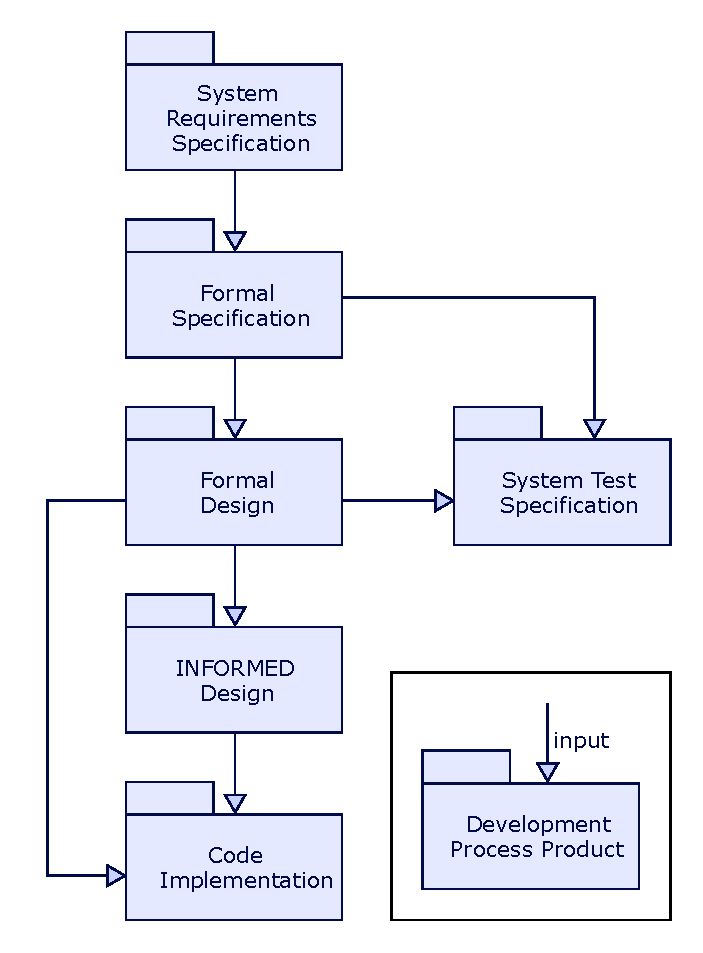
\includegraphics[scale=0.75]{Figures/CbyC_process.pdf}
	\decoRule
	\caption{CbyC development process.}
	\label{fig:CbyCDev}
\end{figure}


\begin{itemize}
	\item r.
\end{itemize}



